\section*{Ziel}

Es werden die Elementarladung $e$  und die \textsc{Avogadro}-Konstante $N_\text{A}$ ermittelt.
\section{Theorie}
\label{sec:Theorie}

Bewegt sich ein Öltröpfen im luftgefüllten Raum, so erfährt es als treibende Kräfte Auftrieb und Gravitation.
Weiterhin wird aufgrund laminarer Luftreibung nach \textsc{Stokes} eine Grenzgeschwindigkeit $v_0$ erreicht.
Bei Erreichen dieser Geschwindigkeit stellt sich ein Kräftegleichgewicht ein,
die Geschwindigkeit $v_0$ ist daher konstant.
Die Bewegungsgleichung für einen solchen Tropfen ist mit
\begin{equation}
	\frac{4\pi}{3}r^3(\rho_\text{Öl}-\rho_\text{Luft})g=6\pi\eta_\text{Luft}v_0
	\label{eq:bewgl_1}
\end{equation}
gegeben, wobei $\rho$ die Dichte, $\eta$ die Viskosität und $r$ der Tröpfenradius ist.
Für den Tröpfenradius $r$ gilt damit sofort
\begin{equation}
	r=\sqrt{\frac{9\eta_\text{Luft}v_0}{g(\rho_\text{Öl}-\rho_\text{Luft})}}.
	\label{eq:radius_v0}
\end{equation}
Befindet sich auf dem Tröpfchen, etwa ausgehend von triboelektrischen Effekten bei der Zerstäubung,
eine Ladung, so reagiert es auf anwesende elektrische Felder.
Im Folgenden wird ein homogenes elektrisches Feld $E$ angenommen, das in oder gegen Fallrichtung des unbeeinflussten Tröpfchens ausgerichtet ist. %; es ist also kollinear zum Lot.
Bei bekanntem elektrischen Feld $E$ muss in der Gleichung \ref{eq:bewgl_1} die zusätzlich auftretende Kraft berücksichtigt werden.
Es gilt hierfür im Allgemeinen
\begin{equation}
	\frac{4\pi}{3}r^3(\rho_\text{Öl}-\rho_\text{Luft})g-6\pi\eta_\text{Luft}v_0= F_\text{el}.
	\label{eq:bewgl_2a}
\end{equation}

\begin{figure}
	\centering
	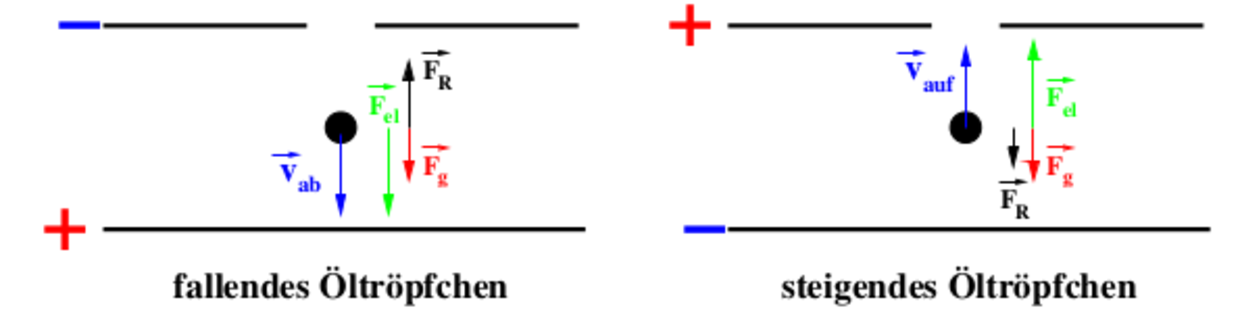
\includegraphics[width=\textwidth]{Bilder/Tropfen.pdf}
	\caption{Kräfte wirken auf ein geladenes Tröpfchen, welches sich im Plattenkondensator befindet.\cite{skript}}
	\label{fig:tropfen}
\end{figure}

Je nach Ausrichtung des Feldes $E$ ist die Bewegung des Tröpfchen in oder gegen Fallrichtung, wie in Abbildung \ref{fig:tropfen} dargestellt..
Hieraus folgen für beide Fälle die Bewegungsgleichungen
\begin{align}
	\frac{4\pi}{3}r^3(\rho_\text{Öl}-\rho_\text{Luft})g-6\pi\eta_\text{Luft}v_\text{ab} &= -q E,\\
	\frac{4\pi}{3}r^3(\rho_\text{Öl}+\rho_\text{Luft})g+6\pi\eta_\text{Luft}v_\text{auf}&= q E.
	\label{eq:bewgl_2}
\end{align}
Mit Hilfe der Geschwindigkeiten kann eine Aussage getroffen werden,
welcher Radius $r$ das gemessene Tröpfchen aufweist und welche Ladung $q$ es trägt.
Es gelten
\begin{equation}
	r=\sqrt{\frac{9\eta_\text{Luft}(v_\text{ab}-v_\text{auf})}{2g(\rho_\text{Öl}-\rho_\text{Luft})}}
	\label{eq:radius}
\end{equation}
und
\begin{equation}
	q=3\pi\eta_\text{L}\sqrt{\frac{9\eta_\text{Luft}(v_\text{ab}-v_\text{auf})}{4g(\rho_\text{Öl}-\rho_\text{Luft})}}\frac{(v_\text{ab}+v_\text{auf})}{E}.
	\label{eq:ladung}
\end{equation}
Durch das Zerstäuben der Öltröpchen ist deren Durchmesser so gering, dass er sich in ähnlichen Größenordnungen bewegt wie die mittlere freie Weglänge der Moleküle in Luft. Die \textsc{Stokes}sche Reibung  $F_{\eta}$ wird hier ungenau und muss durch eine Korrektur behoben werden. Die Viskosität in den Gleichungen \eqref{eq:radius} und \eqref{eq:ladung} wird angepasst. 
Es gilt für die Viskosität in oben beschriebenen Gleichungen
\begin{equation}
	\eta= \eta_\text{Luft}\Bigl(\frac{1}{1+B\sfrac{1}{p r}}\Bigr)
	\label{eq:cunningham}
\end{equation}
mit dem \textsc{Cunningham}-Korrekturterm $B=6.17\cdot 10^{-3}\,\text{Torr}\cdot\text{cm}$ \cite{skript}.

Für die \textsc{Avogadro}-Konstante mit $F=\SI{96485.34}{\coulomb\per\mol}$ \cite{texas_instruments2} gilt
\begin{equation}
	F=N_\text{A}\cdot e,
\label{eq:av}
\end{equation}
sodass diese in der Auswertung bestimmt werden kann, wenn $F$ als gegeben vorausgesetzt und $e$ berechnet wird.
